% Chapter 4
\section{Gripping Algorithm Design} % Main chapter title
\label{Chapter4} % For referencing the chapter elsewhere, use 
The design of the gripping algorithm is critical to the functionality and efficiency of Lasso Gripper, ensuring precise and reliable manipulation of various objects. This section outlines the algorithm's design, which leverages advanced techniques for object recognition and manipulation, ensuring robust performance in diverse scenarios.

% ------------------------- 3.1 Object Recognition and Point Cloud Processing -------------------------
\subsection{}section{Object Recognition and Point Cloud Processing}
The gripping algorithm begins with the recognition of the target object using an Intel REALSENSE depth camera D435i. The camera captures a 3D point cloud of the object, providing detailed spatial information about its shape and orientation. The point cloud data is processed to identify key features of the object, including its boundaries, surface characteristics, and potential gripping points.

\begin{figure}[htbp]
\centering
\begin{tabular}{cc}
\begin{minipage}[t]{0.9\textwidth}
\centering
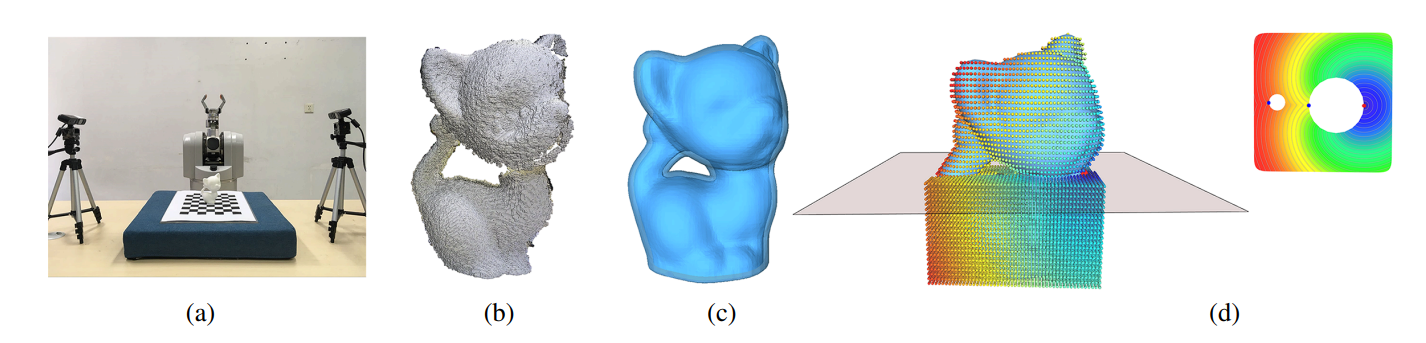
\includegraphics[width=1.0\columnwidth]{Figures/caging.png}
\caption{ The caging loop calculating algorithm for Lasso Gripper \cite{liu2018caging}. (a) The setup of the depth reconstruction system (b)The Point cloud captured by depth camera directly. (c) A r-offset surface is built for defining the grasping space. (d) Two Morse saddle points (blue) are calculated to define the grasping loop.}
\end{minipage}
\end{tabular}
\end{figure}

The algorithm employs a method for identifying the "neck" of the object, which is a critical region for secure gripping. The method entails identifying caging loops, which are closed curves characterized within the embedding space of the target object's shape \cite{liu2018caging}. By decoupling the caging loops from the surface geometry, the algorithm can synthesize feasible caging grasps that are not constrained by the object's surface details. This enables the gripper to handle objects with complex geometries and topologies effectively.

% ------------------------- 3.2 Loop Positioning and Tightening -------------------------
\subsection{Loop Positioning and Tightening}

Once the neck region is identified, the algorithm determines the optimal position for the string loop around the neck. The positioning is crucial for ensuring that the loop can be tightened securely without slipping or causing damage to the object. The algorithm calculates the precise coordinates for the loop's placement, taking into account the object's shape and the desired gripping force.

\begin{figure}[htbp]
\centering
\begin{tabular}{cc}
\begin{minipage}[t]{0.9\textwidth}
\centering
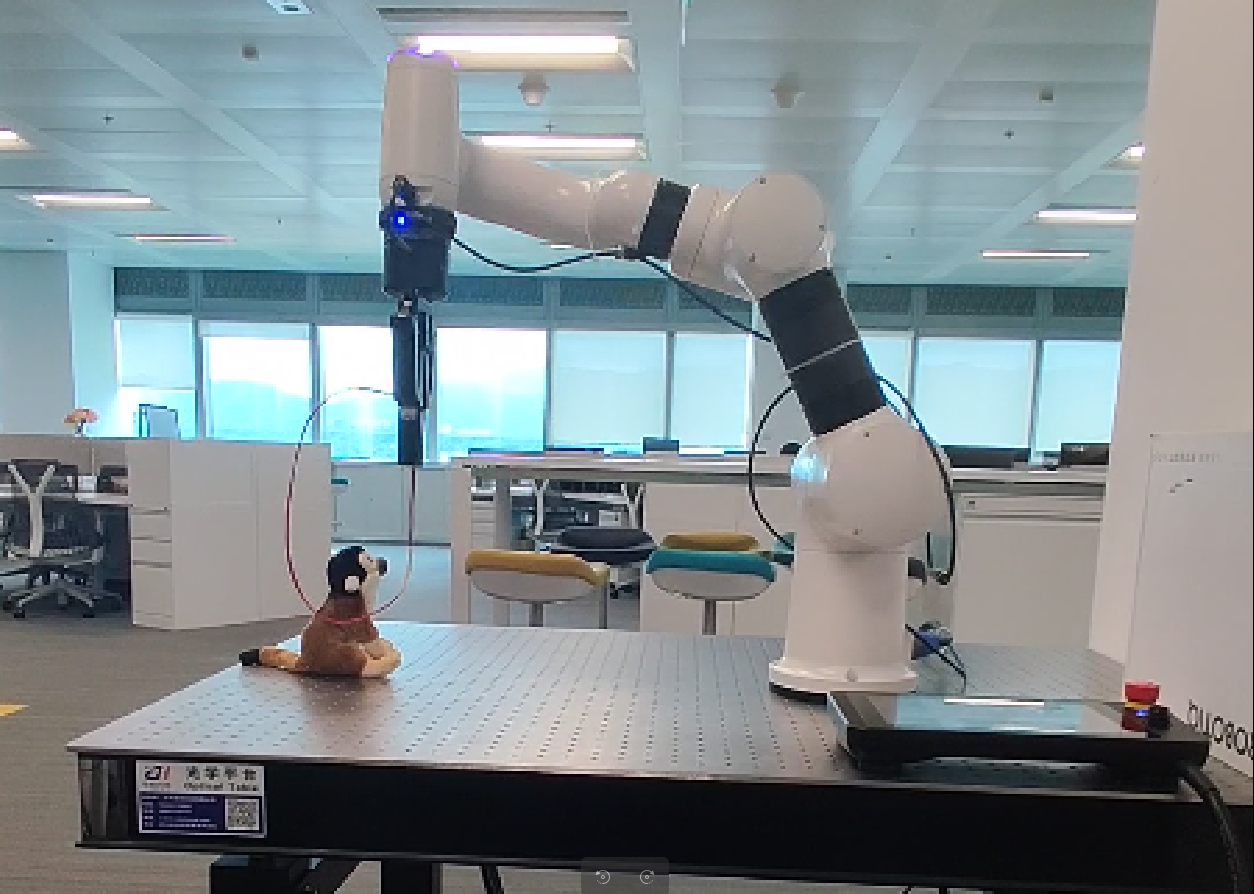
\includegraphics[width=1.0\columnwidth]{Figures/exp.png}
\caption{The illustration of the relative position of the string loop and the target object -- an early test}
\end{minipage}
\end{tabular}
\end{figure}

The tightening process is executed in a controlled manner, with the string loop gradually constricting around the neck region. The wrist of the gripper approaches the object in synchrony with the tightening action, ensuring that the loop maintains its position and grip. The following pseudo code illustrates the sequence of operations:

Input: Point Cloud P, String shooting velocity V

\begin{enumerate}
    \item Scan P using depth camera
    \item Process P to identify key features
    \item Identify neck region N in P using the caging loop method
    \item Determine optimal loop position L according to V 
    \item Align lower end of L with N
    \item Execute controlled tightening action
    \item Approach wrist towards object while maintaining loop position
\end{enumerate}

% ------------------------- 3.3 Real-Time Feedback and Adjustment -------------------------
\subsection{Real-Time Feedback and Adjustment}
The gripping algorithm incorporates real-time feedback mechanisms to adjust the gripping force and position dynamically. Sensors embedded in the gripper provide continuous data on the tension of the string, the position of the loop, and the force exerted on the object. This data is processed by the controller to make real-time adjustments, ensuring that the grip remains secure and stable.

The force feedback sensor, located on the spool's axle, plays a pivotal role in this process. It monitors the tension of the string during the tightening phase and adjusts the motor's torque accordingly. This prevents excessive force that could damage the object and ensures that the grip is firm enough to hold the object securely.
\let\cleardoublepage\clearpage